\documentclass[10pt]{amsart}
\usepackage{graphicx}
\usepackage{amssymb}
\usepackage{amsmath}
\usepackage[utf8]{inputenc}
\usepackage[spanish]{babel}
\newtheorem{theorem}{Theorem}[section]
\newtheorem{lemma}[theorem]{Lemma}
\usepackage{fancyhdr}
\usepackage{tikz}

\theoremstyle{remark}
\newtheorem{remark}[theorem]{Remark}

\numberwithin{equation}{section}

%  Absolute value notation
\newcommand{\abs}[1]{\lvert#1\rvert}

%  Blank box placeholder for figures (to avoid requiring any
%  particular graphics capabilities for printing this document).
\newcommand{\blankbox}[2]{%
 \parbox{\columnwidth}{\centering
%  Set fboxsep to 0 so that the actual size of the box will match the
%  given measurements more closely.
 \setlength{\fboxsep}{0pt}%
 \fbox{\raisebox{0pt}[#2]{\hspace{#1}}}%
}%
}


\begin{document}

\title{Aspectos teóricos relacionados con Teorema de Hahn-Banach}

%  Information for first author
\author{Lester Armando Vallecillo}
%  Address of record for the research reported here
\address{Departamento de Matemáticas, Universidad Nacional Autónoma de Honduras, Francisco Morazán, Tegucigalpa 11101}
\email{lester.vallecillo@unah.edu.hn}

%  Information for second author
%  General info
\date{Diciembre 11, 2019, fue revisado en Diciembre 16, 2019.}
\keywords{Dual, Operador lineal, Extensión, Funcional}

\maketitle

\begin{abstract}
El teorema de Hahn-Banach es uno de los cuatro resultados pilares del análisis funcional que se expone en este articulo para mostrar su utilidad en los diferentes campos de aplicación, y en general del análisis matemático. El presente estudio pretende comprender los aspectos teóricos relacionados con teorema de Hahn-Banach, el cual se enuncia en diferentes versiones, la primera versión es la forma analítica, la segunda es el teorema de extensión y la tercera es la forma geométrica.\\

La versión analítica del teorema de Hahn-Banach propone la extensión de funcionales lineales continuos sobre un espacio vectorial real. Un importante resultado de esta herramienta es el teorema de extensión de Hahn-Banach para espacios normados, el cual propone extender todo funcional lineal continuo definido en un subespacio de un espacio normado a todo el espacio conservando la norma.\\

La versión Geométrica del teorema de Hahn-Banach es también consecuencia de la versión analítica que se centra en resumir distintos teoremas de separación de conjuntos convexos, de los cuales se expone para separación de espacios vectoriales complejos mediante un hiperplano afín que separa dos subconjuntos cualquiera del espacio, de manera similar este teorema se puede aplicar a espacios normados.\\

Particularmente, se propone resolver un problema de mucha relevancia en el origen del análisis funcional, que nace en el estudio de los sistemas de infinitas ecuaciones lineales, denominado problema de los momentos, que esta asociado a una función de distribución de probabilidades del espacio $\mathbb{C}[0,1]$. En su aplicación se ilustra la utilidad del teorema de Hahn-Banach para resolver problemas de infinitas ecuaciones lineales.\\


\end{abstract}


%%%%%%%%%%%%%%%%%%%%%%%%%%%%%%%%%%%%%%%%%%%%%%%%%%%%%%%%%%%%%%55

\section*{Introducción}

La estructura del análisis funcional tiene como base el estudio de espacios de funcionales denominados duales, esto se conoce como teoría de dualidad. A fin de dotar a los espacios fundamentales de algunas propiedades fundamentales, se definen operadores lineales no nulos en el dual que satisfacen determinadas condiciones, principalmente de acotación y por lo tanto, de continuidad, como consecuencia de esta necesidad surge el teorema de Hahn-Banach, formando parte de los cuatro resultados pilares del análisis funcional, el cual se expone explorando la teoría de dualidad sobre los espacios fundamentales, como se ilustra en la Figura \ref{01}.\\ 

\begin{figure}[h]
\centering
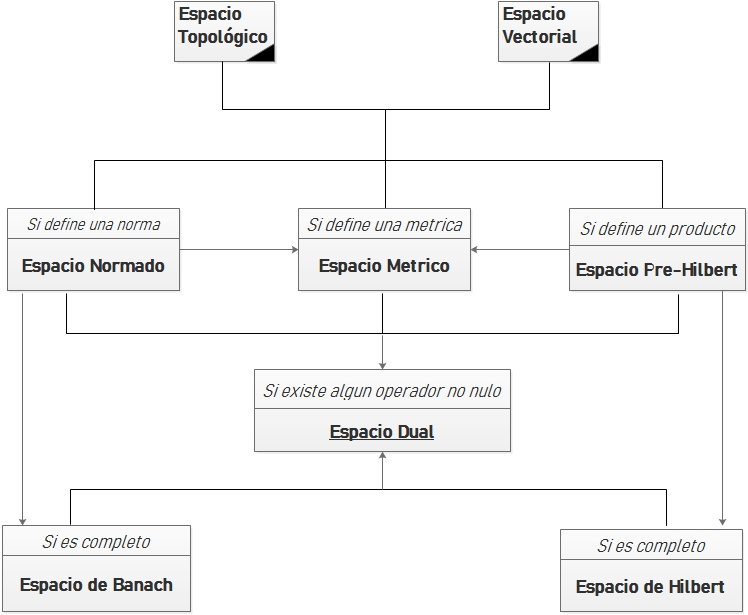
\includegraphics[scale=0.6]{Pic/ESQUEMA01}
\caption{Enfoque de la teoría de dualidad. [Fuente: propia]}
\label{01}	
\hrule
\end{figure}

Fundamentar la teoría de dualidad sugiere tomar como base la definición de los espacios fundamentales descritos en el esquema anterior y enunciar algunos conceptos previos (sección 3.1) para dotar de propiedades a estos espacios utilizando el teorema de Hahn-Banach.\\

La sección \ref{v1} se centra en enunciar la versión analítica del teorema de Hahn-Banach para garantizar la existencia de funcionales lineales continuos no nulos en el dual de espacios fundamentales de dimensión infinita.\\

En la sección \ref{v2} se expone una aplicación de la versión analítica del teorema de Hahn-Banach descrito como el teorema de extensión, para poder dotar a un espacio normado de determinadas propiedades cuando se hace una extensión de un funcional lineal hacia todo el espacio normado por medio de estos funcionales y tratar los problemas de forma general.\\

La versión geométrica del teorema de Hahn-Banach que se describe en la sección \ref{v3}, selecciona un caso de un conjunto de teoremas de separación de espacios. Particularmente, el teorema de separación de espacios vectoriales complejos.\\ \\


%%%%%%%%%%%%%%%%%%%%%%%%%%%%%%%%%%%%%%%%%%%%%%%%%%%%%%%%%%%%%%

\section{Justificación}
En el análisis abstracto del espacio dual ¿ se puede describir topológicamente un espacio normado? Un primer paso sería asegurar la existencia de elementos no nulos en el dual, es decir, un espacio dual no trivial.\\

Se puede asegurar la existencia de funcionales lineales continuos sobre un espacio normado de dimensión finita gracias al Teorema de Tíjonov \cite{ArtAca12}. Sin embargo, no es evidente la existencia de funcionales lineales continuos en espacios normados de dimensión infinita.\\ 

Ciertamente, el análisis funcional tiene mucha importancia cuando se trata de espacios normados de dimensión infinita, de donde surge la idea de extender funcionales lineales de forma que se mantenga una cierta condición de acotación \cite{Rev15}, utilizando conceptos y resultados ya demostrados en los espacios normados de dimensión finita gracias al teorema de Tijonov, y que por lo tanto, garantizan la existencia de funcionales no nulos.\\   

Las propiedades de los espacios normados se enriquecen en el ambiente de los espacios separables, como consecuencia se deduce la versión geométrica del Teorema de Hahn-Banach para concretar distintos resultados de separación de conjuntos convexos. Particularmente, se fortalecen las hipótesis sobre el campo de aplicación y los conjuntos que se pretende separar.\\

De la misma manera, garantizar la existencia de funcionales no nulos en el dual de algunos espacios clásicos como $\mathbb{R}, \ell_p, \ell^\infty$ y $L_p$ entre otros, analizados de manera particular, propone la idea de axiomatizar y resolver estos problemas de forma mas general para espacios fundamentales \cite{ArtAca01}.\\

El teorema de Hahn-Banach está fundamentado en la teoría de dualidad y por su importancia, se extiende a áreas como la teoría de la aproximación, la optimización, análisis complejo, las ecuaciones en derivadas parciales, las finanzas, la termodinámica o la mecánica de fluídos. Sin embargo, se pueden clasificar según el campo de su aplicación: espacios topológicos, retículos vectoriales, módulos, álgebras de Boole, grupos, semigrupos, etc... \cite{Tesis16}.\\

La importancia de describir los aspectos teóricos y enunciar las tres versiones del teorema de Hahn-Banach, radica en analizar algunas variantes y deducir algunos resultados importantes, surge de la necesidad de encontrar nuevas técnicas para abordar una serie de problemas que los métodos tradicionales no podían resolver \cite{ArtAca01}.\\

La utilidad del teorema de Hahn-Banach permite resolver problemas de sistemas lineales de infinitas ecuaciones con infinitas incógnitas, una aplicación particular es el problema de los momentos que esta asociado a un problema de distribuciones de probabilidad, bajo que condiciones se puede asegurar la existencia de un funcional lineal continuo? Se propone definir un funcional de variación acotada y se determinan las condiciones necesarias y suficientes para que el sistema definido en un espacio normado tenga solución.\\ \\

%%%%%%%%%%%%%%%%%%%%%%%%%%%%%%%%%%%%%%%%%%%%%%%%%%%%%%%%%%%%%%%%%%%%
% ------- FIN DE INTRODUCCIÓN --------------------------------------

\section{Antecedentes}

El análisis funcional es una herramienta de mucha utilidad en la ciencia moderna que forma parte del análisis matemático. Surgen los primeros planteamientos del análisis funcional en las funciones definidas sobre ciertos subconjuntos del espacio euclidiano $\mathbb{R}^n$, como elementos de un espacio vectorial y el estudio las ecuaciones diferenciales e integrales que relacionan estos puntos lineales entre estos espacios.\\

Fréchet (1878-1971) desarrolló una teoría abstracta de espacios de funciones, fundamentando el concepto de espacio métrico. Luego, Hilbert (1862-1943) publica una serie de artículos sobre ecuaciones integrales, motivados por los resultados de Fredholm (1866-1927), en conjunto con la tesis doctoral de su alumno Schmidt (1876-1959), nace la teoría actual de espacios de Hilbert con conceptos como bola unidad, convergencia débil, distancia entre elementos, teoría espectral de operadores. Pero, todo ello restringido a las sucesiones de cuadrado sumable $l_2 $.\\

En el siglo XX surge la teoría de integración de Lebesgue(1875-1941). Esta teoría dio paso al estudio de los espacios $L_2[a,b]$, así surge un nuevo problema, ¿qué sucesiones de números reales pueden surgir como los coeficientes de Fourier de alguna función? Fue resuelto por Riesz (1880-1956) y Fischer (1875-1954) de manera independiente, este resultado es hoy día conocido como teorema de Riesz-Fisher y establece que el espacio métrico $L_2[a,b]$ es completo, separable e isométrico al espacio de sucesiones de Hilbert.\\

Por su parte, Riesz propone la representación de cualquier funcional lineal y continuo sobre el espacio $ C[a,b]$, lo que conlleva la ideas intuitiva de dualidad en un espacio, además Riesz es considerado como el padre la teoría abstracta de operadores.\\

En 1920 Stefan Banach (1892-1945) en su tesis doctoral titulada \textit{Théorie des Opérations Linéaries}, define axiomáticamente el espacio vectorial real, normado y ademas completo. Por su parte, presenta otros resultados como el principio de acotación uniforme y el principio de contracción en espacios métricos completos. Lo más importante de la tesis de Banach fue mostrar implícitamente la noción correcta de espacio normado, sujeto a los resultados anteriores de análisis funcional.\\

Ciertamente, Banach resume toda la teoría que se conocía hasta ese momento, incluyendo los tres principios fundamentales del análisis funcional, la teoría de Riesz de operadores, las bases de un espacio normado, la convergencia débil, demostrando parcialmente así, los teoremas de Banach-Alaoglu y Dieudonné \cite{ArtAca03}.\\

En 1933 Mazur dedujo la forma geométrica a partir de la forma analítica, pero no mencionó la posibilidad inversa. En 1941, Dieudonn se refiere a la forma geométrica como el teorema de Hahn-Banach. Bourbaki la llama primero la forma geométrica. La forma analítica es una prima del teorema de Riez de un límite continuo $ f \colon K \rightarrow \left [a, b \right] $ definido en un cerrado El subconjunto $ K $ de un espacio normal $ T $ posee una extensión continua $ F \colon T \rightarrow \left [a, b \right] $ con los mismos límites.\\

 La forma geométrica se asemeja al lema de Urysohn sobre la separación de subconjuntos cerrados disjuntos de un espacio normal por una función continua. El lema de Urysohn generalmente se prueba por inducción, el teorema geométrico de Hahn-Banach por \textit{transfinita} inducción \cite{libro10}.\\

El año 1932 el análisis funcional se consolida como una nueva rama del análisis matemático. Las principales causas fueron la tesis de Banach y el trabajo de Neumann (1903-1957), que propone los fundamentos de la mecánica cuántica. A su vez, se formaliza la teoría abstracta de espacios de Hilbert y la teoría espectral, una de sus grandes deducciones es la equivalencia entre funciones de cuadrado integrable y series de cuadrado sumable, que permite unificar la mecánica matricial y la mecánica ondulatoria.\\

Simultáneamente, Stone (1903-1989), en su libro  \textit{Linear Transformations in Hilbert Space and their Applications to Analysis}, desarrolló la teoría espectral en espacios de Hilbert con aplicaciones al análisis matemático \cite{ArtAca03}. En conclusión, lo que actualmente se conoce como análisis funcional, resulta difícil de resumir en una investigación bibliográfica.\\

Helly en 1912 había planteado el teorema de extensión de Hahn-Banach. investigó las nociones geométricas ligadas a la convexidad, y su relación con la norma. Llevado por esta idea geométrica logro introducir nuevas técnicas de demostración, usando sistemáticamente la separabilidad del espacio y el principio de inducción. Los resultados de Helly fueron fundamentales para la solución general del problema que obtuvo H. Hahn en 1927.\\

La versión analítica del Teorema de Hahn-Banach fue demostrado por el matemático austríaco Hahn en 1927 para un espacio normado definido en un cuerpo de escalares real. Sin embargo, el también austríaco Helly en 1912 había intentado extender un funcional lineal continuo definido en un subespacio de funcionales.\\

Tomando como base el resultado de Hahn, Banach demostró en 1929 un planteamiento más general para un espacio vectorial real, demostrando así que un funcional lineal definido en un subespacio de un espacio vectorial real se puede extender a todo el espacio, preservando la acotación del funcional definido en todo el espacio normado, este resultado se conoce como teorema de extensión.\\

La versión compleja es debida a Bohnenblust y Sobczyk en 1938 y Soukhomlinoff en 1938, de manera independiente que propone cambiar el espacio de escalares real por un espacio complejo \cite{ArtAca01}.\\


Históricamente los teoremas de extensión de Hahn-Banach tienen su raíz en el estudio de los sistemas de infinitas ecuaciones lineales. El problema de resolver un sistema lineal de infinitas ecuaciones e infinitas incógnitas puede entenderse como encontrar un funcional lineal continuo $f$ tal que $f(z_i)=c_i$ con $i=1, 2, 3, .., n$, donde $\{z_i\}$ es una familia de elementos del espacio normado. Un problema particular fue el problema de los momentos. Los primeros desarrollos de la teoría de momentos consistieron en un tratamiento algebraico en el caso particular de momentos: 
\[ {\int_0}^1 t^n d\varphi(t) = c_n\]
para  $i=1, 2, 3, ..., n$, donde
\[\varphi(z_i)= \frac{P'(z_i)}{P(z_i)}\]

donde $P(z_i)$ es polinomio de grado $n$. En 1839 Sturm (1803-1855), Sylvester (1814-1897) y Bochard (1817-1880) trabajaron en este problema, que equivale al problema de descomposición de $\varphi(z_i)$ en fracciones simples \cite{Lib20}.\\  



\section{Aspectos Teóricos}
Se considera que el lector tiene conocimiento de los conceptos básicos del análisis funcional, como la definición de los espacios fundamentales y/o clásicos. Partiendo de está base, y por lo visto en el esquema estructural de enfoque teórico del análisis funcional relacionado al teorema de Hahn-Banach, descrito en la sección anterior, se definen tales conceptos para enunciar el teorema de Hahn-Banach.\\

En la Figura \ref{02} se ilustra una abstracción de la teoría de dualidad como base del análisis funcional y como el proceso para fundamentar los aspectos teóricos centrando su análisis en el teorema de Hahn-Banach.\\ 
\begin{figure}[h]
\centering
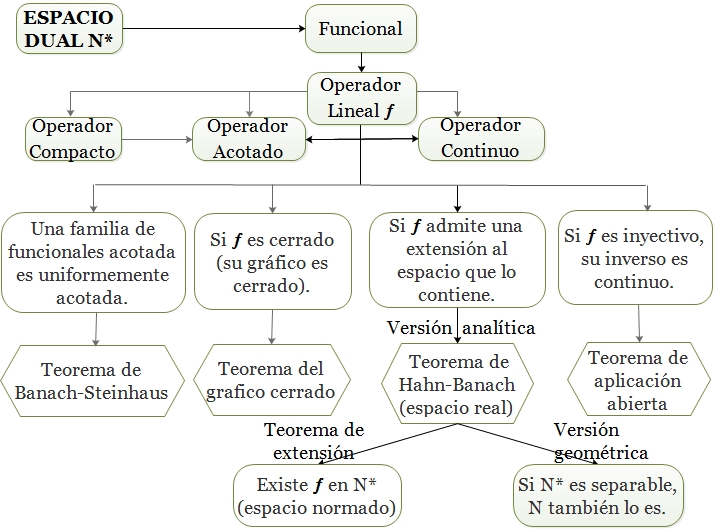
\includegraphics[scale=0.7]{Pic/Esquema02}
\caption{Enfoque de abstracción de la teoría de dualidad en el análisis funcional. [Fuente: propia] \label{02}}	
\hrule
\end{figure}\\ \\


\subsection{Conceptos previos} \ \\ \\
%%%%%%%%%%%%%%%%%%%%%%%%%%%%%%%%%%%%%%%%%%%%%%%%%%%%%%%%%%%%%%%%
Se definen algunos conceptos básicos del análisis funcional utilizados para enunciar el teorema de Hahn-Banach. Según el esquema anterior, son los siguientes:

\subsubsection{Operador lineal} \cite{Cur05} \\
Es una aplicación ó transformación lineal continua $f:\mathbb{V} \longrightarrow \mathbb{Y}$ entre espacios vectoriales topológicos. Se puede clasificar como:\\
\renewcommand{\descriptionlabel}[1] %
{\hspace*{0.5cm}\textit{#1}}
\begin{description}
\item[Operador Compacto: ] es un operador lineal definido sobre un subconjunto de un espacio normado, tal que su imagen es un conjunto compacto.\\

\item[Operador Acotado: ] es una aplicación lineal definida entre espacios normados, tal que la norma puede acotarse. Es decir, existe $k>0$: $\parallel f(x) \parallel \leq k \parallel x \parallel$, $ \forall x \in \mathbb{V}$.\\ \item[Operador Continuo: ] un operador lineal es continuo si y solo si es acotado.\\
\end{description} En consecuencia de la definición de operador lineal, surge algunos conceptos importantes del análisis funcional y utilizados en el teorema de la versión analítica(real) del teorema de Hahn-Banach.\\ 
\subsubsection{Funcional lineal} \ \\
Es un operador lineal definido en un espacio arbitrario sobre algún espacio como cuerpo de escales.\\

\subsubsection{Funcional Sublineal} \ \\ Es un funcional lineal $p:\mathbb{V} \longrightarrow \mathbb{K} $ con las propiedades siguientes:\\

\begin{tabular}{l  c r}
subaditiva: & \hspace*{1cm} $ p(x + y) = p(x)+ p(y)$ & \\
positivamente homogénea: & $p(\alpha x)(x)= \alpha p(x) $ & $ \forall x \in \mathbb{V}$\\[0.8cm]
\end{tabular} 

Se dice que un funcional lineal $f:\mathbb{V} \longrightarrow \mathbb{K} $ está \textbf{dominado} por $p$ si,
\[f(x) \leq p(x) \hspace*{1cm} \forall x \in \mathbb{V} \] 

\subsubsection{Espacio Dual} \cite{Web17}\\ Sea $\mathbb{V}$ espacio vectorial sobre un cierto cuerpo $ \Bbbk $, el espacio dual $\mathbb{V}$* es el conjunto de todas los funcionales lineales sobre $ \Bbbk $, con las propiedades siguientes:
\[(\phi + \psi)(x)=\phi (x)+\psi (x) \]
\[(a\phi )(x) = a\phi(x) \]

para todos $\phi$, $\psi$ en $\mathbb{V}$*, $a$ en $ \Bbbk $ y $x$ en $\mathbb{V}$. %%%%%%%%%%%%%%%%%%%%%%%%%%%%%%%%%%%%5
\subsubsection{Elemento maximal} \ \\
Un elemento $m \in A$ se llama elemento maximal de $A$ si $m \leq x$ implica que $a = x$, $\forall x \in A$
\subsubsection{Orden parcial} \cite{Web17} \\ Un orden parcial es una relación binaria $R(\leq)$ sobre un conjunto $\mathbb{V}$ que es reflexiva, antisimétrica, y transitiva, es decir, para cualesquiera $a$, $b$, y $c$ en $\mathbb{V}$ se tiene que: \begin{itemize}
\item $aRa$ (reflexividad).
\item Si $aRb$ y $bRa$, entonces $a = b$ (antisimetría). \item Si $aRb$ y $bRc$, entonces $aRc$ (transitividad). \end{itemize} 
\subsubsection{Variedad afín} \ \\ $\mathbb{S} \subset \mathbb{V}$, es una variedad afín si $\mathbb{S} = x_0 + M$, donde $x_0$ es un vector y $M \subset \mathbb{V}$.

\subsubsection{hiperplano afín} \ \\
Si $M$ es un subespacio maximal, se dice que $\mathbb{S}$ es un hiperplano afín.

\subsubsection{Subconjunto absorbente} \ \\ Diremos que A es absorbente si en $R^{+}$, se cumple que $A = X$, es decir, si $\forall x \in \mathbb{V}$, $\exists \alpha > 0$ tal que $\lambda x \in A$ para todo $\alpha \in \mathbb{C}$ con $\mid \lambda \mid \leq \alpha $. \subsection{Lema de Zorn} \ \\
Sea $(A;\leq)$ un conjunto parcialmente ordenado e inductivo y sea$a \in A$. Entonces existe $m$ elemento maximal en A.


\subsection{Versión analítica del teorema de Hahn-Banach}\label{v1} \cite{ArtAca01}\\ \\ Para garantizar la existencia de un funcional lineal continuo no nulo en un espacio normado, se toma en cuenta que la continuidad de un funcional lineal no nulo en un espacio normado equivale a su acotación en la bola unitaria. Por tanto, se propone extender un funcional lineal de forma que se mantenga una cierta condición de acotación, esto se puede hacer sustituyendo la norma por algún funcional. Esta idea es conocida como la versión real del teorema de Hahn-Banach.\\

\subsection*{Teorema 1 (Teorema de Hahn-Banach, versión analítica)} \ \\
Sean un $f: \mathbb{V} \longrightarrow \mathbb{R}$ un funcional lineal sobre un espacio vectorial real $\mathbb{V}$ a un cuerpo de escalares real $\mathbb{R}$, $ \mathbb{S} \subseteq \mathbb{V}$ un subespacio y $f \in \mathbb{S}$* un funcional lineal dominado por un funcional sublineal $p$ (ver la Figura \ref{03}) y que cumple la acotación:\\
\[f(y) \leq p(y) \hspace*{1cm} \forall y \in \mathbb{S} \]

Entonces existe un funcional $\phi \in \mathbb{V}$*
que cumple las condiciones siguientes:\\
\begin{tabular}{l r}
$ \phi(x) \leq p(x)$ & $ \forall x \in \mathbb{V}$\\
$\phi$ extiende a $f$, entonces, $\phi(y) = f(y)$ & $\forall y \in \mathbb{S}$.\\[0.6cm]
\end{tabular} Es decir, 
\[%
\begin{array}[c]{c c c c c c l}%
\phi: & \mathbb{V} & & & \phi \leq p            & & \\
& \mid & \searrow & &                   & \Longrightarrow & \phi(y) = f(y)\\ 
f: & \mathbb{S} & \longrightarrow & \mathbb{R} & f \leq p & & \end{array} \]\\

%%%%%%%%%%%%%%%%%%%%
La demostración de este resultado esta basada en el lema de Zorn. En primera instancia, se considera una colección de subconjuntos $\{(\mathbb{Y}, \phi)\}$ parcialmente ordenados con $\mathbb{Y} \supset \mathbb{S}$ subconjunto de un espacio vectorial real $\mathbb{V}$, un funcional lineal $\phi$ definido en $\mathbb{S}$, que extiende a $f$ y esta dominado por $p$ \cite{ArtAca01}.\\

En fin, por el lema de Zorn, se afirma que la familia de los pares ordenados $\{(\mathbb{Y}, \phi)\}$ posee un elemento maximal ($\mathbb{S}$, $\phi$), esto verifica que todo $(\mathbb{Y}, \phi) \geq (\mathbb{S}, p)$. En segunda instancia, se demuestra que $\mathbb{Y} = \mathbb{V}$, de donde se deduce que $\phi(y) = f(y)$. El proceso usual de su demostración, se describe a continuación: \cite{Lib19}\\ 
\begin{enumerate}
\item Se considera el conjunto $\mathbb{Y}$ de todas las extensiones lineales $\phi$ de $f$ que satisfacen $\phi(x) \leq p(x)$ sobre el dominio $\mathbb{S}$ que puede ser parcialmente ordenado y por el lema de Zorn
existe un elemento maximal con un funcional $f \in \mathbb{Y}$*.

\item Se prueba que $f$ esta definido en todo el espacio $\mathbb{V}$. \item Luego se deduce una relación auxiliar que se usará en el paso 2. 

\item Para completar la prueba, se deduce que $\mathbb{Y} = \mathbb{V}$.\\
\end{enumerate} 
Sin embargo, no se pretende demostrar el teorema, solamente se pretende describir los aspectos teóricos relacionados con teorema de Hahn-Banch.\\



Geometricamente, se puede pensar en un subconjunto compacto de un espacio topológico, que mediante un funcional lineal que se extiende a todo el espacio, bajo la condición de acotación de un funcional sublineal, es decir, que el funcional lineal $f$ esta dominado por el funcional sublineal $p$, como se muestra en Figura \ref{03}.\\
\begin{figure}[h]
\centering 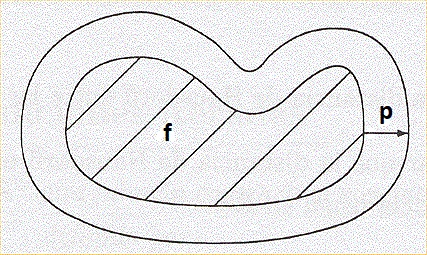
\includegraphics[scale=0.92]{Pic/Esquema05.jpg}
\caption{Descripción geométrica de la extención de un funcional lineal $f$ dominado por un funcional sublineal p. [Fuente: propia]}\label{03}	
\hrule
\end{figure} \vspace*{1cm}	


%%%%%%%%%%555%%%%%%%%
\subsection*{Teorema de Hahn-Banach para espacios complejos}
\ \\ \\
Para analizar la versión analítica del teorema de Hahn-Banach en espacios complejos, se necesita principalmente algunas propiedades de valor absoluto, es decir, su norma. De esta manera, se remplaza la norma del cuerpo de escalares de números reales por la norma de números complejos.\\ 

\subsection*{Corolario 1.1 (Teorema de Hahn-Banach, caso complejo)} \ \\ Sea $\mathbb{V}$ es un espacio vectorial complejo, $\mathbb{S}$ subconjunto de $\mathbb{V}$ y una \textit{seminorma}\footnote{Note que la seminorma es un funcional sublineal.} $p \in \mathbb{V}$*, de modo que $ \forall x \in \mathbb{V} $, se cumple que $ \left \vert f(x) \right \vert \leq p(x) $,  entonces existe $\phi: \mathbb{V} \to \mathbb{C}$ funcional lineal continuo que extiende a $f$ y $\forall x \in \mathbb{V}$, se cumple que,

\[ \left \vert \phi(x) \right \vert \leq p(x) \].\\ \subsection{Teorema de extensión en espacios normados}\label{v2} \cite{libro10}\\ \\
La noción de espacio locamente convexo es la generalización mas adecuada de espacio normado. Este resultado hace que el teorema de Hahn-Banach sea objeto de algunos estudios dentro del análisis funcional en espacios normados, el cual es fundamental por su importancia en la teoría de los operadores lineales y continuos \cite{ArtAca03}.\\ \subsection*{Teorema 2 (Teorema de Hahn-Banach, versión de extensión)} \ \\ 
Sea $ X $ es espacio normado sobre $ K = \mathbb{R} $ o $ \mathbb{C}$ y $ f \colon \mathbb{S} \to K $, es decir, $f \in \mathbb{S}$* es un funcional lineal continuo, entonces existe un funcional continuo $ \phi \in \mathbb{X}$* que extiende a $ f $ definido en todos los $ X $ de manera que $\forall x \in X$, se cumple que,

\[ \left \Vert \phi(x) \right \Vert = \left \Vert f(x) \right \Vert \]\\

El teorema de extención de Hahn-Banach establece la posibilidad de extender todo funcional lineal continuo definido en un subespacio de un espacio normado a la totalidad del espacio, conservando ademas la misma norma.\\

\subsection{Versión geométrica del teorema de Hahn-Banach}\label{v3}
\cite{libro10}\\ \\ La versión geométrica del teorema de Hahn-Banach es también conocida como teorema de separación de espacios. Consiste en la separación de conjuntos convexos, de los cuales se expone la separación de espacios vectoriales reales o complejos, aplicando la versión analítica del teorema de Hahn-Banach. De manera similar, se aplica en separación de subconjuntos en algunos espacios fundamentales como los espacios normados y se extiende una serie de consecuencias interesantes.\\ 

Si $\mathbb{V}$ es un espacio vectorial topológico real o complejo, y una variedad lineal afín $ \mathbb{S} = x_0 + M $ subconjunto de $\mathbb{V}$, no cumple con la convexidad abierta, entonces existe un hiperplano cerrado $H$ que contiene a $\mathbb{S}$ y separa dos subconjuntos cualquiera.


\subsection*{Teorema 3 (Teorema de Separación, versión geométrica)} \ \\ Sean $\mathbb{V}$ espacio vectorial complejo, $A$ y $B$ subconjuntos convexos, no vacíos, disjuntos. Si existe $ x_0 \in A$ tal que $ A-x_0 $ es absorbente. Entonces se puede separar $A$ y $B$, si existe $f: X \longmapsto \mathbb{K}$ y $ \sigma \in \mathbb{R} $, tales que, 
\[f(a) \leq \sigma \leq f(b)\] $\forall a \in A$, $\forall b \in B$.

En consecuencia, con el teorema de separación se interpreta que los subconjuntos convexos $A$ y $B$ se separan mediante el hiperplano afín de la ecuación siguiente: 

\[f(x) =\alpha\]

Dicho de otra manera el hiperplano separa, dejando a un lado al conjunto $A$ y al otro a $B$, de esto se deduce la separación de subconjuntos convexos en espacios normados utilizando el teorema de Hahn-Banach \cite{ArtAca01}.\\[0,8cm]




%%%%%%%%%%%%%%%%%%%%%%%%%%%%%%%%%%%%%%%%%%%%%%%%%%%%%%%%%%%%%%%%
%     APLICACIÓN
%%%%%%%%%%%%%%%%%%%%%%%%%%%%%%%%%%%%%%%%%%%%%%%%%%%%%%%%%%%%%%%%%

\section{Aplicación al problema de los momentos}\cite{ArtAca01}\\ \\
Los teoremas de extensión de Hahn-Banach tienen su raíz en el estudio de los sistemas de infinitas ecuaciones lineales. Para ver la conexión, consideremos un sistema de m ecuaciones lineales con n incógnitas,

\[ a_{i1}x_1+a_{i2}x_2+a_{i3}x_3+ . . . + a_{in}x_n = c_i \]
para $i=1, 2, 3, ..., n$. Es decir,  \[\sum_{i=1}^{n} \sum_{j=1}^{n} a_{ij}x_j = c_i \] para $j=1, 2, 3, ..., n$.
Para encontrar una solución utilizando el teorema de Hahn-Banach, si se logra encontrar el dual no trivial de un espacio normado, con el cuerpo de escalares $\mathbb{K}^n$, entonces se identifica el funcional siguiente: \[ f(a_{i1}, a_{i2}, a_{i3}, ..., a_{in})=c_i \] 
para  $i=1, 2, 3, ..., n$. De la misma manera, puede entenderse como encontrar un funcional lineal continuo $f$ tal que $f(z_i)=c_i$, donde $\{z_i\}$ es una familia de elementos del espacio normado, el cual tiene alguna condición de dependencia lineal. Un ejemplo del problema anterior es el llamado \textit{problema de los momentos}.\\
\subsection{Problema de momentos} \cite{Lib20}\\

En la formulación del problema de momentos se considera una función no decreciente $\varphi(t)$, es decir, con medida no negativa $d \varphi(t)$. Se llaman momentos de $\varphi(t)$ a los valores $c_n$, tales que $c_n$ existe para $n=1, 2, 3, ...$ y se cumple que,

\[c_n = {\int_a}^b t^n d\varphi(t) \]

Algunos problemas de momentos mas comunes son los siguientes: \begin{itemize}
\item Si $(a,b)$ = $(0,\infty)$ se considera problema de momentos de Stieltjes.

\item Si $(a,b)$ = $(-\infty,\infty)$ se considera problema de momentos de Hamburger.

\item Si $(a,b)$ = $(0,1)$ se considera problema de momentos de Hausdorff.\\

\end{itemize} 
\subsubsection{Problema de momentos de Hausdorff} \cite{ArtAca21}\\

Una versión general del llamado problema de momentos plantea que, dada una sucesión $\{c_n\}$ con $n=1, 2, 3, ...$, donde $c_n \in \mathbb{K}$, se propone encontrar una función $\varphi$ de variación acotada en $[0, 1]$.\\

Este problema aparece en diversos planteamientos tanto matemáticos como físicos, en particular está muy relacionado con la teoría de polinomios ortogonales. Por ejemplo, el problema de los momentos puede estar asociado a un problema de distribuciones de probabilidad, si se toma una sucesión de números reales $\{c_n\}$, bajo qué condiciones se puede asegurar la existencia de un funcional lineal continuo? El primer paso es definir un funcional en el espacio $C[0, 1]$, es decir, asegurar la existencia de una función de variación acotada $ \varphi(t) $ de forma que, para cada $n \in N$ se cumple:

\[ c_n = {\int_0}^1 t^n d\varphi(t) \]

En el problema anterior se dan condiciones necesarias y suficientes para que un sistema de infinitas ecuaciones e infinitas incógnitas en un espacio normado tenga solución. Este resultado, es consecuencia del teorema de Hahn-Banach, de donde se establece la siguiente relación de equivalencia.
\subsubsection*{\textbf{Teorema 4.1:} Las siguientes afirmaciones son equivalentes:} 

\begin{itemize} 
\item $c \in C^{*}[0, 1]$.
\item Existe $\varphi: [0, 1] \to \mathbb{C}$ de variación acotada, tal que $c(f) = {\int_0}^1 f(t) d \varphi(t)$,\\
donde la integral es la integral de Riemann-Stieltjes, ademas $\lVert c \lVert$ es la variación.\\
\end{itemize}
Por tanto, el problema de los momentos se puede plantear en nuevos términos, encontrar $c \in C^{*}[0, 1]$, tal que $c(t^n) = c_n$
para $n=1, 2, 3, ...$.\\

 El problema general de momentos no tiene solución, pero el teorema de Hahn-Banach permite dar la siguiente caracterización.\\
\subsubsection*{\textbf{Teorema 4.2:}} Sean $(X, \lVert \rVert)$ un espacio normado sobre $\mathbb{K}$, $(c_\alpha) \subset \mathbb{K}$ con $\alpha \in \varOmega$, $(x_\alpha) \subset X$. Las siguientes afirmaciones son equivalentes:\\
\begin{description} 
\item[i)] $c \in X^{*}$, tal que $c(x_\alpha) = c_\alpha$ para todo $\alpha \in \varOmega$.
\item[ii)] Existe una constante $M>0$ tal que 
\[\mid \sum_\alpha a_\alpha c_\alpha \mid \leq M \lVert a_\alpha x_\alpha \rVert\] donde la suma se realiza sobre los subconjuntos finitos no vacíos de $\varOmega$.\\ 
\end{description}


Para demostrar $i) \to ii)$, se toma la hipótesis $c(x_\alpha) = c_\alpha$, y se remplaza en la sumatoria al lado izquierdo de la desigualdad anterior. Es decir,

\[\mid \sum_\alpha a_\alpha c_\alpha \mid = \lVert \sum_\alpha a_\alpha c(x_\alpha) \rVert \]

Ademas,

\[\lVert \sum_\alpha a_\alpha c(x_\alpha) \rVert = \mid c \sum_\alpha a_\alpha x_\alpha \mid \]
Entonces,
\[\mid c \sum_\alpha a_\alpha x_\alpha \mid \leq \lVert c \rVert \lVert \sum_\alpha a_\alpha x_\alpha \rVert \]\\

Por lo tanto, 
\[\mid \sum_\alpha a_\alpha c_\alpha \mid \leq M \lVert a_\alpha x_\alpha \rVert\] 

Si se toma $M= \lVert c \rVert$ se encuentra la variación acotada de $\varphi(t)$, donde la suma se realiza sobre los subconjuntos finitos no vacíos de $\varOmega$.\\ 

Esto demuestra que la relación de equivalencia $i) \to ii)$, la segunda relación se deja como tarea al lector.\\ 


El resultado anterior responde nuestra hipótesis planteada para este problema. En conclusión, si se puede asegurar la existencia de un funcional lineal continuo de variación acotada, bajo las condiciones establecidas en los incisos de los teoremas 4.1 y 4.2.

\newpage
\section{Conclusiones}
El análisis funcional tiene como base la teoría de la dualidad, es decir, su estudio se centra en la abstracción del funcionales lineales que forman el espacio dual no trivial.\\

El teorema de Hahn-Banach es uno de los 4 resultados pilares del análisis funcional utilizado en muchos campos de estudio par resolver problemas reales.\\

Los operadores lineales del dual se pueden extender con el propósito de dotar de propiedades más generales a los espacios fundamentales.\\

Los espacios normados se pueden enriquecer de atributos mediante la extención de funcionales lineales con cierta condición de acotación.\\

El teorema de Hahn-Banach fue demostrado primero en su versión analítica para espacios definidos sobre el cuerpo de escalares real(posteriormente, complejo), luego Banach generalizo este concepto a espacios normados.\\ 

Se pueden resolver sistemas de infinitas ecuaciones lineales utilizando el teorema de Hahn-Banach, un aplicación particular es el problema de los momentos, que propone encontrar un funcional de variación acotada.\\

El teorema de Hahn-Banach se centra en encontrar algún funcional definido en un subconjunto y sujeto a condiciones de acotación.\\

Una idea intuitiva del teorema de Hahn-Banach es sustituir la norma es remplazar la norma en un espacio normado por un operador lineal.\\

La noción de espacio locamente convexo es la generalización mas adecuada de espacio normado.\\

A futuro se espera estudiar aplicaciones del teorema de Hahn-Banach en la áreas de computación, mecánica cuántica y economía.\\ \\

\newpage
\bibliographystyle{amsplain}
\begin{thebibliography}{20}


\bibitem [01]{ArtAca01} Juan Carlos Cabello Píñar(2009), \textit{Análisis Funcional} , Universidad de Granada \textbf{vol. II}, Capitulo 2, pag. 33-55.\\

\bibitem [02]{Libro02}Banach, S.(1987), \textit{Theory of Linear Operations}, Amsterdam, North Holland.\\

\bibitem [03]{ArtAca03}Bombal, Fernando(2003), \textit{Análisis funcional: una perspectiva histórica}, Universidad de Sevilla , Sevilla, España.\\

\bibitem[04]{Rev04}Bryan, P. Rynne, Martin, A. Youngson](2000), \textit{Linear Funtional Analysis}, II edición, Department of Mathematics and the Maxwell Institute for Mathematical Sciences, Heriot-Watt University, Escocia.\\

\bibitem[05]{Cur05}Antonio Vera Lopez y Pedro Alegria Ezquerra, \textit{Un Curso de Análisis Funcional}, Universidad del Pais Vasco, España.\\

\bibitem[06]{Libro06}Alejandro A. Fúster y Lucia A. Cortes(2005), \textit{Teoría, procedimientos de demostración y ejercicios de Análisis Funcional}, Universidad Central “Marta Abreu” de Las Villas Cuba, Cuba, 2005.\\

\bibitem[07]{07}Diestel, J.(1975), \textit{Geometry of Banach Spaces: Selected Topics, Springer-Verlag}, New York, E.U.A.\\

\bibitem[08]{08}Gaughan, E.(1972), Introducción al análisis, Alhambra. Madrid.\\

\bibitem[09]{libro10}Narici, Lawrence, \textit{On the Hahn-Banach Theorem}, New York, E.U.A.\\

\bibitem[10]{ArtAca12}Fuster, E. Llorens(2003), \textit{Análisis funcional}, Universidad de Sevilla , Sevilla, España.\\

\bibitem[10]{Web16}\textit{Las matemáticas de la cuántica}, http://www.fisicacuantica.es/las-matematicas-de-la-cuantica/\\

\bibitem[11]{Web17}\textit{Análisis funcional}
https://es.wikipedia.org/wiki/AnC3A1lisisfuncional\\

\bibitem[12]{Rev15}Jiménez Sevilla, \textit{Algunos conceptos básicos del Análisis Funcional}, Universidad Complutense de Madrid, Facultad de Ciencias Matemáticas, Madrid, España.\\

\bibitem[13]{Tesis16}Diaz, Remedios M.(2015), \textit{El teorema de Hahn-Banach}, Universidad La Laguna, San Cristóbal de La Laguna,España.\\

\bibitem[14]{ArtAca17}Gutierréz, José Adalid(1982), \textit{On the boundedness of the Banach space-valued Hilbert transform}, The University of Texas at Austin, Department of Mathematics, Austin, Texas, E.U.A.\\

\bibitem[15]{ArtAca18}Stojanoff, Demetrio(2015), \textit{Un Curso de Análisis Funcional}. \\

\bibitem[16]{Lib19}Gil P., Eddison(2016), \textit{Teorema de Lax-Milgran y una aplicación a las ecuaciones diferenciales}, Universidad Distrital Francisco José Caldas, Bogotá, Colombia.

\bibitem[17]{Lib20}Paolini, Graciela B.(1995), \textit{Un estudio sobre el problema de los momentos y la solución de una aplicación a la teoría de control.}, Instituto de Matemática de Bahía Blanca, Argentina.

\bibitem[18]{ArtAca21}Miana, Pedro J.(2006), \textit{Análisis Funcional}, Departamento de Matemáticas
Universidad de Zaragoza, España.

\end{thebibliography}

\newpage
\thispagestyle{empty}

\textbf{Euclides:\\}
\begin{center}
	\textit{Las leyes de la naturaleza no son más que los pensamientos matemáticos de Dios.}
	\vspace*{17cm}
\end{center}

\end{document}

%------------------------------------------------------------------------------
% End of journal.tex
%------------------------------------------------------------------------------